\documentclass[tikz,border=2pt]{standalone}
\usepackage[T1]{fontenc}
\usepackage[scaled]{helvet}
\renewcommand{\familydefault}{\sfdefault}
\usepackage{tikz}
\usetikzlibrary{external,calc,shapes.callouts,shapes.arrows}
\usetikzlibrary{arrows.meta,patterns,patterns.meta,shapes.arrows}
\usetikzlibrary{decorations.pathreplacing}
\tikzset{>=Latex,
  max width/.style args={#1}{
    execute at begin node={\begin{varwidth}{#1}},
    execute at end node={\end{varwidth}}
  }
}
\usetikzlibrary{shapes}
\usetikzlibrary{external}
\begin{document}
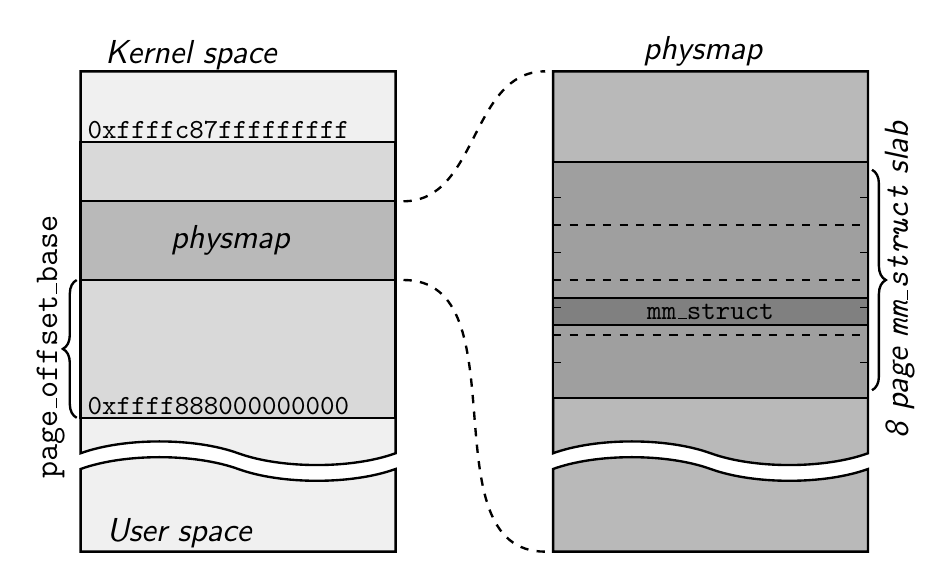
\begin{tikzpicture}

    \tikzstyle{upper}+=[
        line width = 0.3mm,
        tape,
        draw,
        tape bend top=none,
        tape bend height=3mm,
        tape bend bottom=out and in,
        minimum width=4cm,
        minimum height=5cm,
        fill=gray!12
    ]
    \tikzstyle{lower}+=[
        line width = 0.3mm,
        tape,
        draw,
        tape bend top=none,
        tape bend height=3mm,
        tape bend bottom=out and in,
        minimum width=4cm,
        minimum height=1.2cm,
        fill=gray!12,
        rotate=180
    ]
    \tikzstyle{dpmrange}+=[
        draw,
        line width = 0.3mm,
        minimum width=4cm,
        minimum height=3.5cm,
        fill=gray!30
    ]
    \tikzstyle{dpm}+=[
        draw,
        line width = 0.3mm,
        minimum width=4cm,
        minimum height=1cm,
        fill=gray!55
    ]
    \tikzstyle{objbool}+=[
        draw,
        line width = 0.3mm,
        minimum width=4cm,
        minimum height=3cm,
        fill=gray!75
    ]
    \tikzstyle{obj}+=[
        draw,
        line width = 0.22mm,
        minimum width=4cm,
        minimum height=0.35cm,
        fill=gray
    ]
    \tikzstyle{arrow}+=[
        -{Latex[length=2mm]},
        rounded corners=0.7mm,
        line width = 0.2mm
    ]
    \tikzstyle{iline}+=[
        dashed,
        rounded corners=0.7mm,
        line width = 0.3mm
    ]
    \tikzstyle{pageline}+=[
        iline,
        line width = 0.18mm
    ]

    % ----------------------------------------------------------------------------
    \coordinate(kernel) at (0,-0.5);
    \coordinate(user) at (0,-3.8);
    \coordinate(range) at (0,-0.8);
    \coordinate(dpm) at (0,-0.3);
    \coordinate(dpmup) at (6,-0.5);
    \coordinate(dpmdown) at (6,-3.8);
    \coordinate(objbool) at (6, -0.8);
    \coordinate(obj) at (6, -1.2);
    \draw[decorate,decoration={brace,amplitude=5pt},line width=0.3mm] ([shift=(range)]-2.05,-1.75) -- ([shift=(dpm)]-2.05,-0.5);
    \draw[decorate,decoration={brace,amplitude=5pt},line width=0.3mm] ([shift=(objbool)]2.05,1.4) -- ([shift=(objbool)]2.05,-1.4);

    % ----------------------------------------------------------------------------
    \node[upper] at (kernel) {};
    \node[lower] at (user) {};
    \node[dpmrange] at (range) {};
    \node[dpm] at (dpm) {};
    \node[upper,fill=gray!55] at (dpmup) {};
    \node[lower,fill=gray!55] at (dpmdown) {};
    \node[objbool] at (objbool) {};
    \node[obj] at (obj) {};

    % ----------------------------------------------------------------------------
    \draw[iline] ([shift=(dpm)]2.1,0.5) to [out=0, in=180] ([shift=(dpmup)]-2.1,2.35);
    \draw[iline] ([shift=(dpm)]2.1,-0.5) to [out=0, in=180] ([shift=(dpmdown)]-2.1,-0.45);

    % ----------------------------------------------------------------------------
    \node[font=\ttfamily] at ([shift=(range)]-0.25,1.9) {0xffffc87fffffffff};
    \node[font=\ttfamily] at ([shift=(range)]-0.25,-1.6) {0xffff888000000000};
    \node[font=\ttfamily\large,rotate=90] at ([shift=(dpm)]-2.38,-1.35) {page\_offset\_base};
    \node[font=\itshape\large,rotate=90] at ([shift=(objbool)]2.4,0) {8 page \texttt{mm\_struct} slab};
    \node[font=\itshape\large] at ([shift=(dpm)]-0.1,0) {physmap};
    \node[font=\itshape\large] at ([shift=(kernel)]-0.6,2.55) {Kernel space};
    \node[font=\itshape\large] at ([shift=(user)]-0.75,-0.22) {User space};
    \node[font=\itshape\large] at ([shift=(dpmup)]-0.1,2.6) {physmap};
    \node[] at ([shift=(obj)]0,0) {\texttt{mm\_struct}};

    % ----------------------------------------------------------------------------
    \draw[pageline] ([shift=(objbool)]-2,0) to ([shift=(objbool)]2,0);
    \draw[pageline] ([shift=(objbool)]-2,0.7) to ([shift=(objbool)]2,0.7);
    \draw[pageline] ([shift=(objbool)]-2,-0.7) to ([shift=(objbool)]2,-0.7);
    \draw[pageline] ([shift=(objbool)]-2,1.05) to ([shift=(objbool)]-1.8,1.05);
    \draw[pageline] ([shift=(objbool)]2,1.05) to ([shift=(objbool)]1.8,1.05);
    \draw[pageline] ([shift=(objbool)]-2,-1.05) to ([shift=(objbool)]-1.8,-1.05);
    \draw[pageline] ([shift=(objbool)]2,-1.05) to ([shift=(objbool)]1.8,-1.05);
    \draw[pageline] ([shift=(objbool)]-2,0.35) to ([shift=(objbool)]-1.8,0.35);
    \draw[pageline] ([shift=(objbool)]2,0.35) to ([shift=(objbool)]1.8,0.35);

    % ----------------------------------------------------------------------------
    \draw[pageline] ([shift=(objbool)]-2,-0.35) to ([shift=(objbool)]-1.8,-0.35);
    \draw[pageline] ([shift=(objbool)]2,-0.35) to ([shift=(objbool)]1.8,-0.35);

\end{tikzpicture}
\end{document}
